\section{Using Additional Data}\label{sec:useadddata}

Since dialogue summarization data is limited, researchers 
adopt data augmentation or borrow datasets from other tasks. 
We divide the data into two categories: 
Narrative Text and Dialogues.

\subsection{Narrative Text}

A number of {narrative text corpora} are utilized to do language modeling and learn commonsense knowledge which is shared across tasks.
Since most of today's summarization models are based on pre-trained encoder-decoder models, such as BART~\cite{lewis2020bart}, PEGASUS~\cite{zhang2020pegasus}, and T5~\cite{raffel2020exploring},  \textbf{common crawled text corpora} can be regarded as the backbone corpora of dialogue summarization. It generally includes Wikipedia, BookCorpus~\cite{zhu2015aligning} and 
C4~\cite{raffel2020exploring}. 
These pre-trained models, such as GPT-3~\cite{brown2020language}, can be directly used for dialogue summarization with prefix-tuning approaches~\cite{prodan2021prompt}.
%\KZ{citet usually produces more than one author, so pls use 
%plural form.}
\citet{li2021learn} transformed such data by dividing the sequence 
into two spans, selecting span pairs with higher overlaps by Rouge scores for training their model with better copying behaviors.
Overlapped text generation task is proposed which uses the first span to generate the second span. It further boosts their proposed model with the correlation copy mechanism on both document and dialogue summarization tasks, which copies words from $D$ on better occasions during the summary generation.


%\KZ{You use too many ``utilize'''s everywhere. It's not a very good word
%and should be avoided if possible.}
Document summarization is the most similar task to dialogue summarization. As a result, \textbf{document summarization data} are a natural choice for learning the summarization ability.
\citet{zhang2021exploratory} show that BART pre-trained with 
CNN/DM~\cite{hermann2015teaching}~\footnote{\url{https://huggingface.co/facebook/ bart-large-cnn}} enhances the dialogue summarization in the meeting and drama scenarios.
CNN/DM, Gigaword~\cite{rush2015neural}, and 
NewsRoom~\cite{grusky2018newsroom} were all adopted to train a model from scratch by~\citet{zou2021low}.
For taking advantage of models trained document summarization data and doing zero-shot on dialogues, \citet{ganesh2019restructuring} narrowed down the format gap between documents and dialogues by restructuring dialogue to document format with complicated heuristic rules, such as discourse labels mentioned in Section~\ref{sec:graphs}
Differently, \citet{zhu2020end} shuffled sentences from multiple 
documents to get a simulated dialogue for pre-training, including 
CNN/DM, XSum~\cite{narayan2018don} and NYT~\cite{evan2008nyt}.
Similarly, \citet{park2022leveraging} simulated dialogues based on each document with three transformation functions: arranging text into dialogue format by adding ``Speaker 1:'', shuffling sentence order and omitting the most extractive sentence for enhancing the abstractiveness of constructed samples.


\textbf{Commonsense knowledge data} are also welcomed since it is a
basis for language understanding.
\citet{khalifa2021bag} considered three reasoning tasks, including ROC stories 
dataset~\cite{mostafazadeh2016corpus} for short story ending prediction, 
CommonGen~\cite{lin2020commongen} for generative commonsense reasoning, 
and ConceptNet for commonsense knowledge base construction. 
These three tasks, together with dialogue summarization, are jointly trained with multi-task learning and show a performance boost.
%@article{liu2004conceptnet,
%	title={ConceptNet—a practical commonsense reasoning tool-kit},
%	author={Liu, Hugo and Singh, Push},
%	journal={BT technology journal},
%	volume={22},
%	number={4},
%	pages={211--226},
%	year={2004},
%	publisher={Springer}
%}

Besides, MSCOCO~\cite{lin2014microsoft} as a \textbf{short text corpus} is used in~\citet{zou2021low} for training the decoder with narrative text generation ability.


\subsection{Dialogue}

For collecting or constructing more \textbf{dialogue summarization data} 
without the need for human annotations, data augmentation approaches are 
proposed. \citet{liu2021controllable} and \citet{khalifa2021bag} augmented 
by replacing person names in both the dialogue and the reference summary 
at the same time. These augmented data are definitely well-paired and 
are preferred to mixing with the original data during fine-tuning. 
\citet{jia-etal-2022-post} simply paired the whole dialogue with each summary sentence and further trained the model with a prefix-guided generation task before fine-tuning, where the first several tokens of the target sentence are provided for guiding the model on generation and learning to rephrase from dialogue to narrative text to some extent.
\citet{asi2022end} shows that it is possible to take advantage of giant language models such as GPT-3~\cite{brown2020language} to collect pseudo summaries by inputting dialogues with pre-defined question hints.
\citet{liu2022data} collects augmented training pairs with a small seed dataset by following steps: aligning summary spans with utterances, replacing utterances by reconstruction of the masked dialogue,
and filling up the masked summary given the augmented dialogue. 
All these three steps are done with trained models on other tasks having sufficient data.
\cite{fang2022spoken} augmented and refined the original training pairs with an utterance rewriter model~\cite{liu2020incomplete} and a coreference resolution model~\cite{joshi2020spanbert}, leading to understandable dialogues.
Besides, using relatively large-scaled crawled dialogue summarization data as 
a pre-training dataset, such as MediaSum~\cite{zhu2021mediasum}, 
for other low-resource dialogue summarization scenarios was considered in \citet{zhu2021mediasum}'s work. 
For crawled data without summaries, pseudo summaries are constructed by selecting leading comments from the long forum threads on the Reddit~\cite{yang2022tanet}.




Other \textbf{dialogue data} without paired summary are also valuable.
\citet{feng2020dialogue} took questions as outputs and a number of utterances after each question as inputs, regarding question generation as the pre-training objective to help identify important contents in downstream summarization. 
\citet{khalifa2021bag} adopted word-level masks mentioned 
before on PersonaChat~\cite{zhang2018personalizing} and Reddit comments 
for fine-tuning. 
\citet{qi2021improving} pre-trained with dialogues from MediaSum and TV4Dialogue besides document summarization datasets used in \cite{zhu2020end}. They also stitch dialogues randomly to simulate topic transitions. 
\citet{zhong2021dialoglm} proposed a generative pre-training framework for long dialogue understanding and comprehension. Different from BART, Pegasus or T5 pretrained on general common crawled text, DialogLM in this paper is pretrained on dialogues from MediaSum dataset and OpenSubtitles Corpus~\cite{lison2016opensubtitles2016}. It corrupts a window of dialogue utterances with dialogue-inspired noises, similar to the noising operations mentioned in Section~\ref{sec:designselftasks}. 
The original window-sized utterances are the recovering target based on the remaining dialogue. Such a window-based recovering task is proposed to be more suitable for dialogues considering its scattered information and highly content-dependent utterances. 
Besides, \citet{amanda-etal-2022-shift} took advantage of a self-annotated corpus based on SAMSum~\cite{gliwa2019samsum} which converts each utterance individually to a third-person rephrasing.
They showed benefits on the same dataset under the zero-shot setting by pre-training with the perspective shift corpus.
%It recovers the original dialogue utterances in a window based on the dialogue-inspired noises, 
%The difference is that these operations are only performed on utterances or words in a window of $D$, 
%because the information in dialogues are more scattered than 
%in documents and \KZ{recovering snippets is more meaningful for dialogues}. 
%Finally, the model can be fine-tuned for downstream dialogue summarization tasks. 


Furthermore, \citet{zou2021low} broke the training for dialogue summarization 
model into three parts, namely encoder, context encoder and decoder, 
to train the dialogue modeling, summary language modeling and 
abstractive summarization respectively. 
Dialogue corpus, short text corpus, and summarization corpus were all 
used in this work, helping to bridge the gap between out-of-domain 
pre-training and in-domain fine-tuning, especially for low-resource settings.
	
\subsection{Summary and Opinions}

\begin{figure}
	\centering
	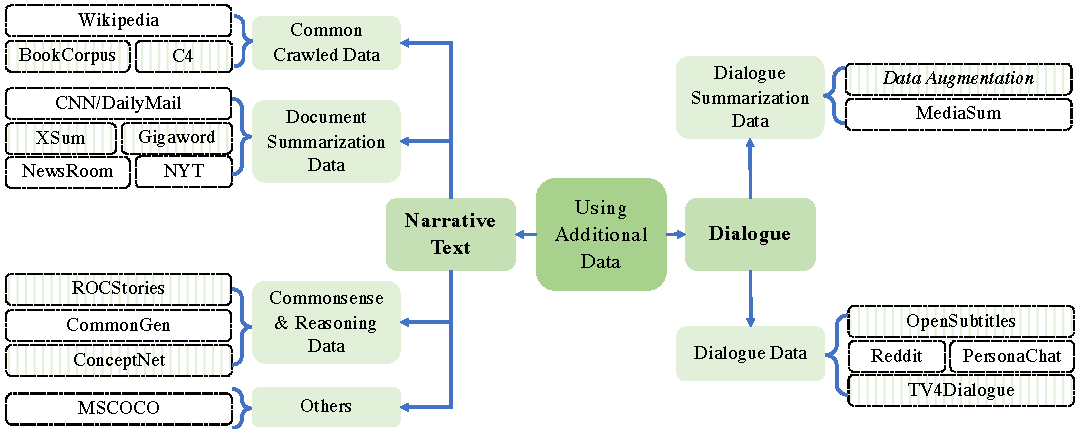
\includegraphics[scale=0.7]{fig/approach-data.pdf}
	\caption{A summary of additional data.}
	\label{fig:app-data}
\end{figure}

Additional data in previous work are summarized in Figure~\ref{fig:app-data}. These data are always used in the following ways:
\begin{itemize}
	\item \textbf{Pre-training with corresponding training objectives}. 
Common crawled text data, document summarization data and dialogue data are 
mostly used in this way~\cite{zou2021low}, where the language styles or data 
formats are quite different from dialogue-summary pairs. It hopes to 
provide a better initialization state of the model for dialogue summarization. 
On the other hand, It is also a good way of coarse-to-fine-grained training, 
where pre-training is done with the noisy data by data augmentation or from other 
domains and fine-tuning with the oracle dialogue summarization training data~\cite{feng2020dialogue,zhu2021mediasum}.


\item \textbf{Mixing with dialogue summarization training data} and 
training for dialogue summarization directly. 
Data here are usually more similar to dialogue-summary pairs obtained by data 
augmentation~\cite{liu2021controllable,khalifa2021bag} or with intensive 
commonsense~\cite{khalifa2021bag,liu2022data}. 
\end{itemize}

The advantages and disadvantages of using additional data are as follows:
\begin{itemize}
	\item[\Checkmark] The language understanding ability among different 
corpora is the same intrinsically. As a result, additional data helps 
dialogue summarization, especially in low-resource settings, 
which further alleviates the burden of summary annotation by humans.
	\item[\Checkmark] The intensive knowledge in specially designed 
corpora helps strengthen the dialogue summarization model. 
	\item[\Checkmark] The additional unlabeled data can be trained 
with self-supervised tasks mentioned in Section~\ref{sec:designselftasks} for 
better performance.
	\item[\XSolidBrush] Training with additional data makes significant improvements while requiring 
more time and computational resources, demonstrating the sample inefficiency of current dialogue summarization models.
	\item[\XSolidBrush] Training with more data is not always effective~\cite{zhang2021exploratory,nair2021data}, especially when the divergence between 
the additional corpus and original dialogue summarization corpus is huge.  Elaborate data augmentation approaches avoid this problem when training data is not too scarce.
\end{itemize}
	
